% Filename: Results
% Last update: Monday, 1/31/2019 by Ally Warner
%
%%%%%%%%%%%%%%%%%%%%%%%%%%%%%%%%%%%%%%%%%%%%%%%%%%%%%%%%%%%%%%%%%%%%%%

\section{Results \& Discussion}
\label{sec:results}

The open-source dataset that was released with this paper includes raw image data, image acquisitions, and preprocessed/corrected images for all image modalities along with all of the necessary inputs and outputs for preprocessing/correction steps of the pipeline. We also include the raw and preprocessed EEG signal data along with the scripts used to obtain and process the data. We included all intermediate steps in the dataset as well, such as the complete, high-resolution brain segmentation that can be used to create three-dimensional tetrahedral volume and surface meshes. We provide two three-dimensional tetrahedral finite element meshes made from the segmentation of different resolutions that serve as volume conductors to solve forward and inverse EEG problems along with the sizing fields used to generate them. We also provide simulation examples of the EEG forward problem, with isotropic and anisotropic systems; functional image data mapped onto a tetrahedral mesh; electroencephalography (EEG) signals mapped onto net electrodes; and diffusion tensor data. 

All SCIRun networks used to generate results and the open-source dataset is available at \url{www.sci.utah.edu/SCI_headmodel}. 

\subsection{Diffusion Tensor Images}

To add anisotropy to the forward problem simulations, which creates more accurate results, we generated a tensor field of the white matter tracts. Figure \ref{fig:tensorvis} and Figure \ref{fig:tensorvis2} show the anisotropy in a typical axial cross section slice calculated from the preprocessed DWIs using equation \ref{eq:scaling}. The anisotropy of the white matter is represented by ellipsoids (Figure \ref{fig:tensorvis2} ). The direction and radius of the ellipsoid correspond to the eigenvector and eigenvalue of the anisotropy tensor for each voxel, respectively. The RBG color maps to the XYZ direction of the primary eigenvector.               

\begin{figure}[H]
\begin{center}
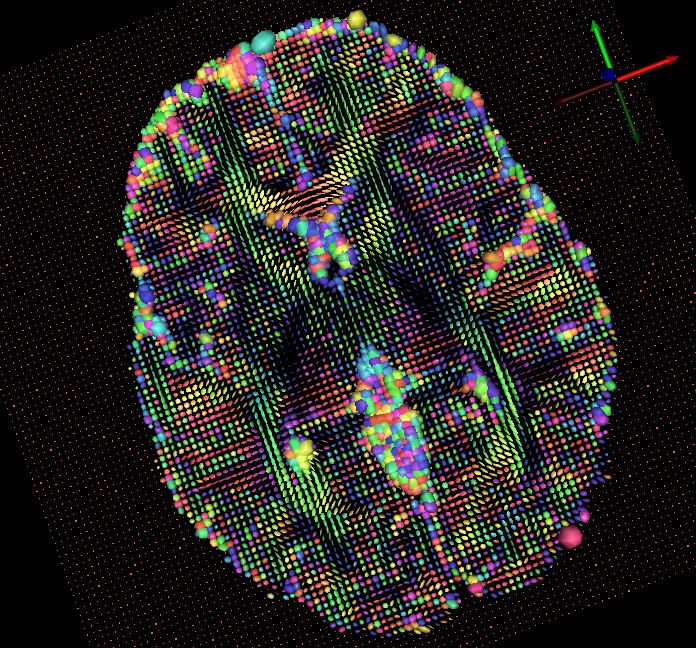
\includegraphics[width=0.75\textwidth]{Figures/DTI_1.png}
\caption{Diffusion tensor visualization using SCIRun.}
\label{fig:tensorvis}
\end{center}
\end{figure}

\begin{figure}[H]
\begin{center}
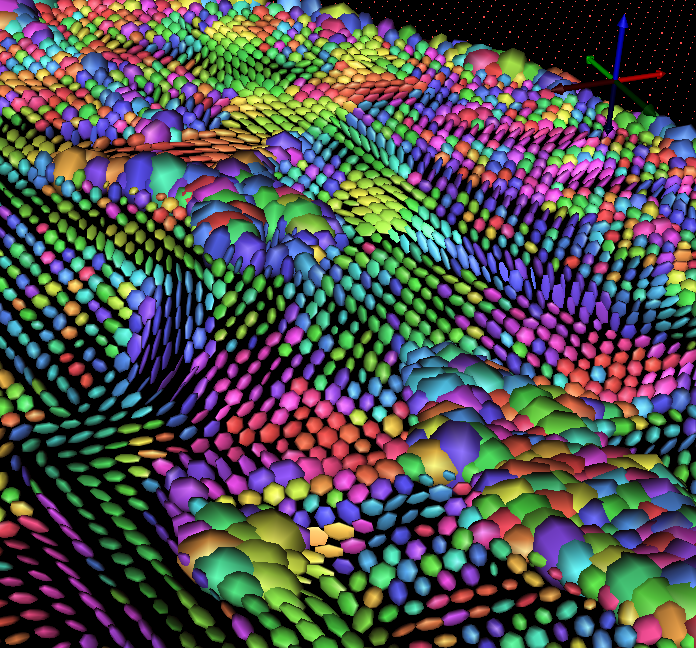
\includegraphics[width=0.75\textwidth]{Figures/DTI_2.png}
\caption{Diffusion tensor visualization using SCIRun.}
\label{fig:tensorvis2}
\end{center}
\end{figure}

The manual registration we applied to the diffusion tensor data, described in Section \ref{sec:reg}, aligned well with the cortical mesh (Figure \ref{fig:dtireg} (\textit{left})). Figure \ref{fig:tensorvis} shows more anisotropy throughout white matter and less anisotropy throughout the gray matter and CSF. However, there is noise around the outside of the axial slice from imperfect alignment.  
 
We chose to build the tensor field in SCIRun rather than in 3D Slicer \cite{ref:slicer} or FSL DTIFIT, which are common software packages for building brain tensor fields, because the orientation of data from these softwares differed in orientation when compared to SCIRun. It made for difficult registration to the cortical surface mesh, which we were performing using SCIRun. Tensor orientation is important when registering to diffusion data and can be difficult to correctly register. We registered other datatypes to the diffusion tensor coordinate space to ensure the tensor orientation was correct. When we built the tensor field in SCIRun and put it back into 3D Slicer, the data's orientation appeared upside down and backwards (Figure \ref{fig:backwards}) from what we saw in SCIRun. To apply a correct and accurate registration, we used the outputs of DTIFIT in SCIRun as explained in Section \ref{sec:reg}.

\begin{figure}[H]
\begin{center}
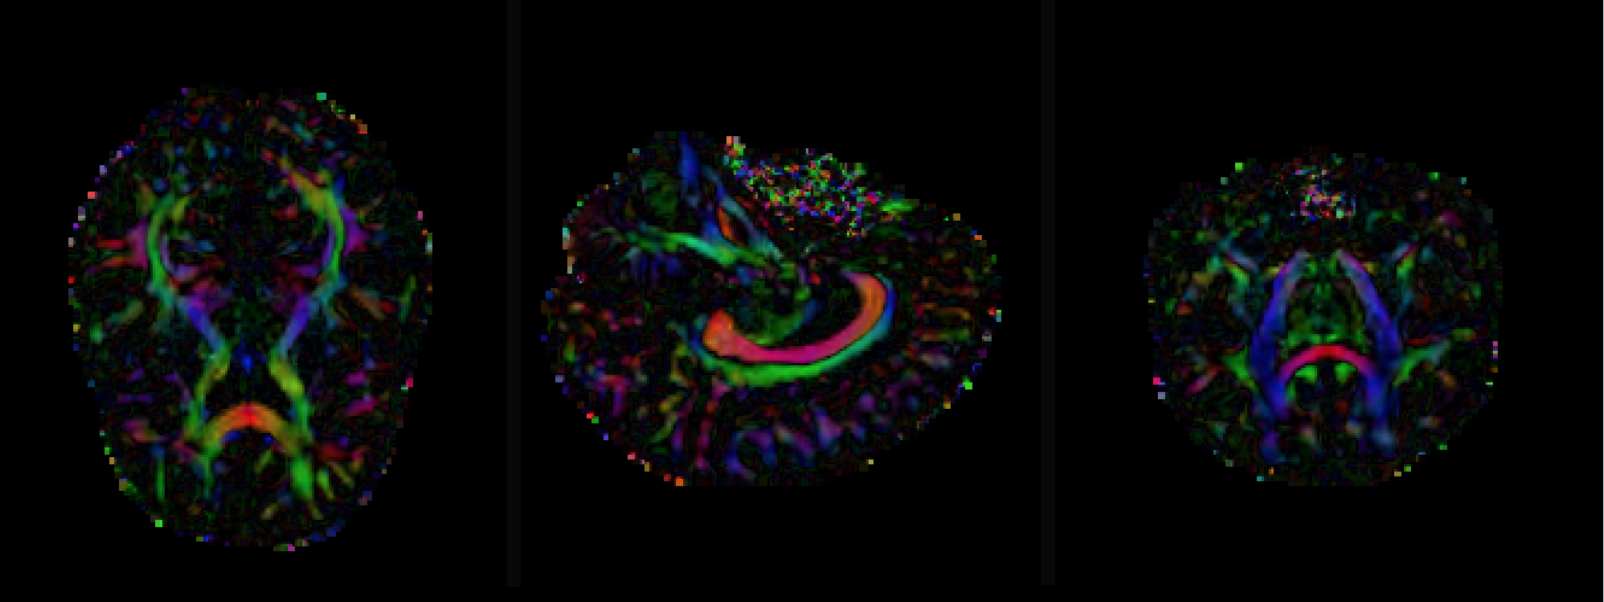
\includegraphics[width=0.75\textwidth]{Figures/backwards.png}
\caption{Example of difference in orientation between SCIRun and 3D
  Slicer data.}
\label{fig:backwards}
\end{center}
\end{figure}

\subsection{Segmentation}

For this project, we segmented the head into eight detailed layers (Figure \ref{fig:fullseg}), listed in Section \ref{sec:Seg}. We used this segmentation to create an inhomogeneous three-dimensional tetrahedral mesh.

\begin{figure}[H]
\begin{center}
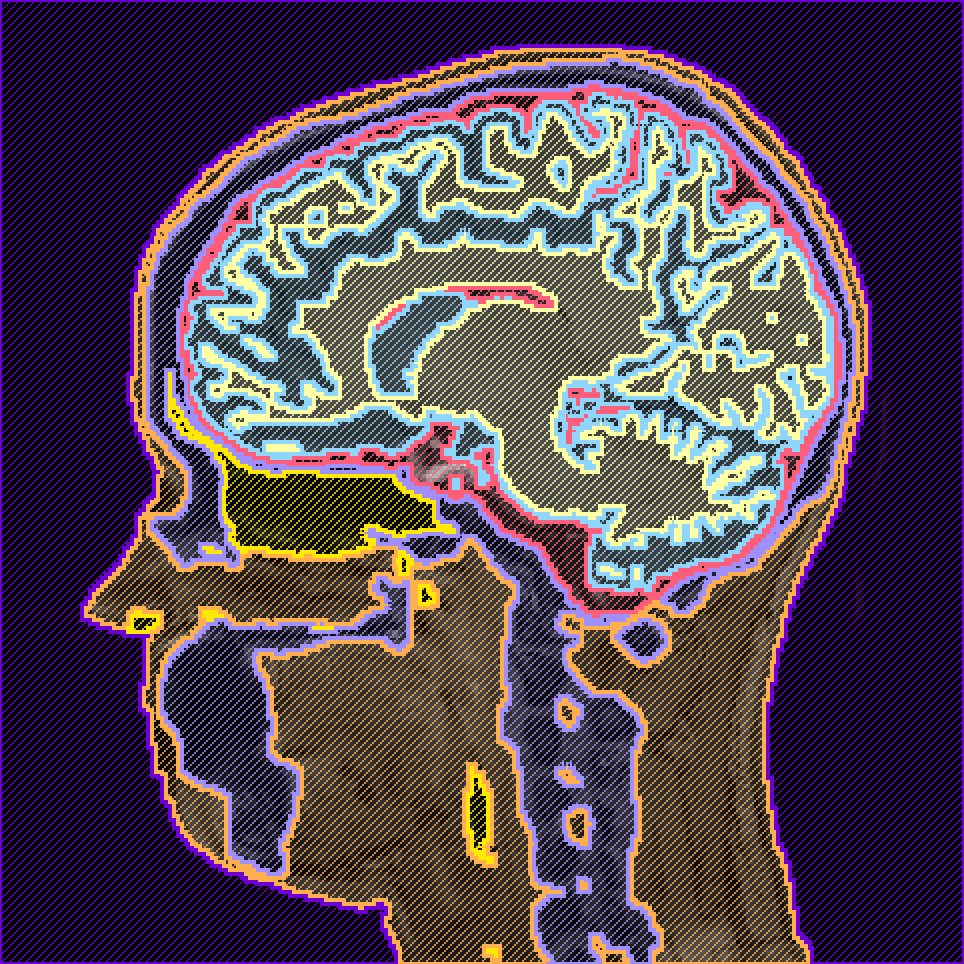
\includegraphics[height=2.35in]{Figures/seg_1}
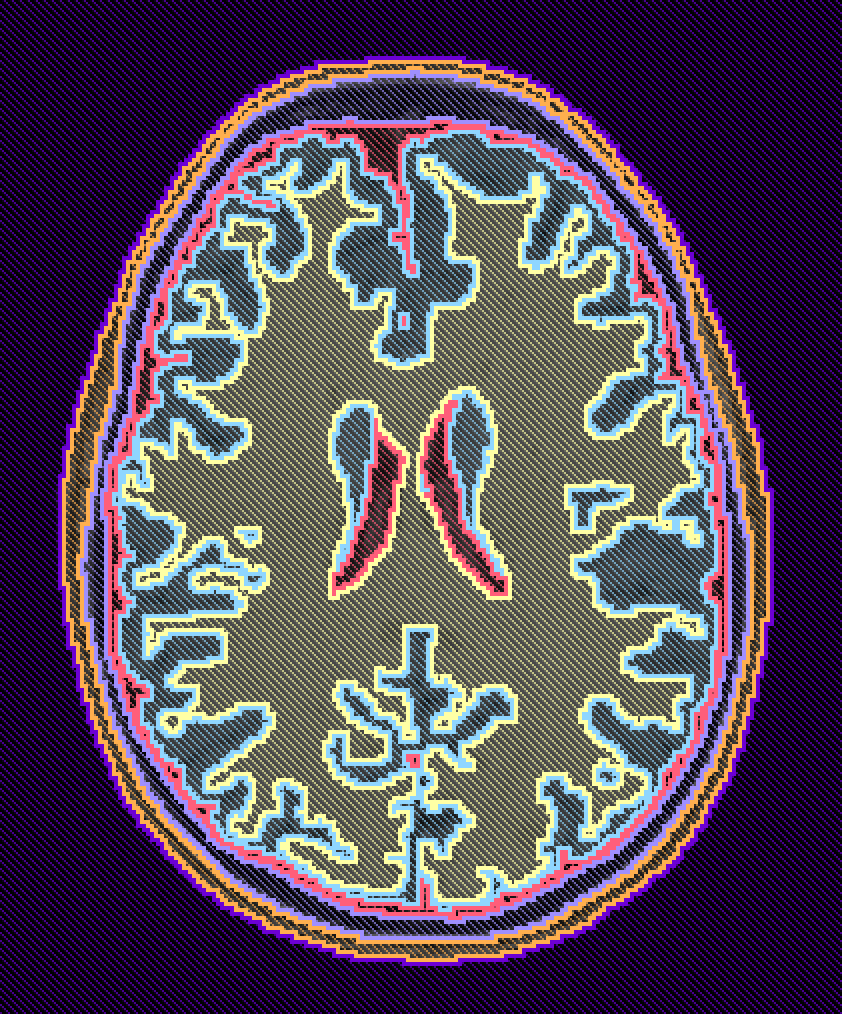
\includegraphics[height=2.35in]{Figures/seg_2}
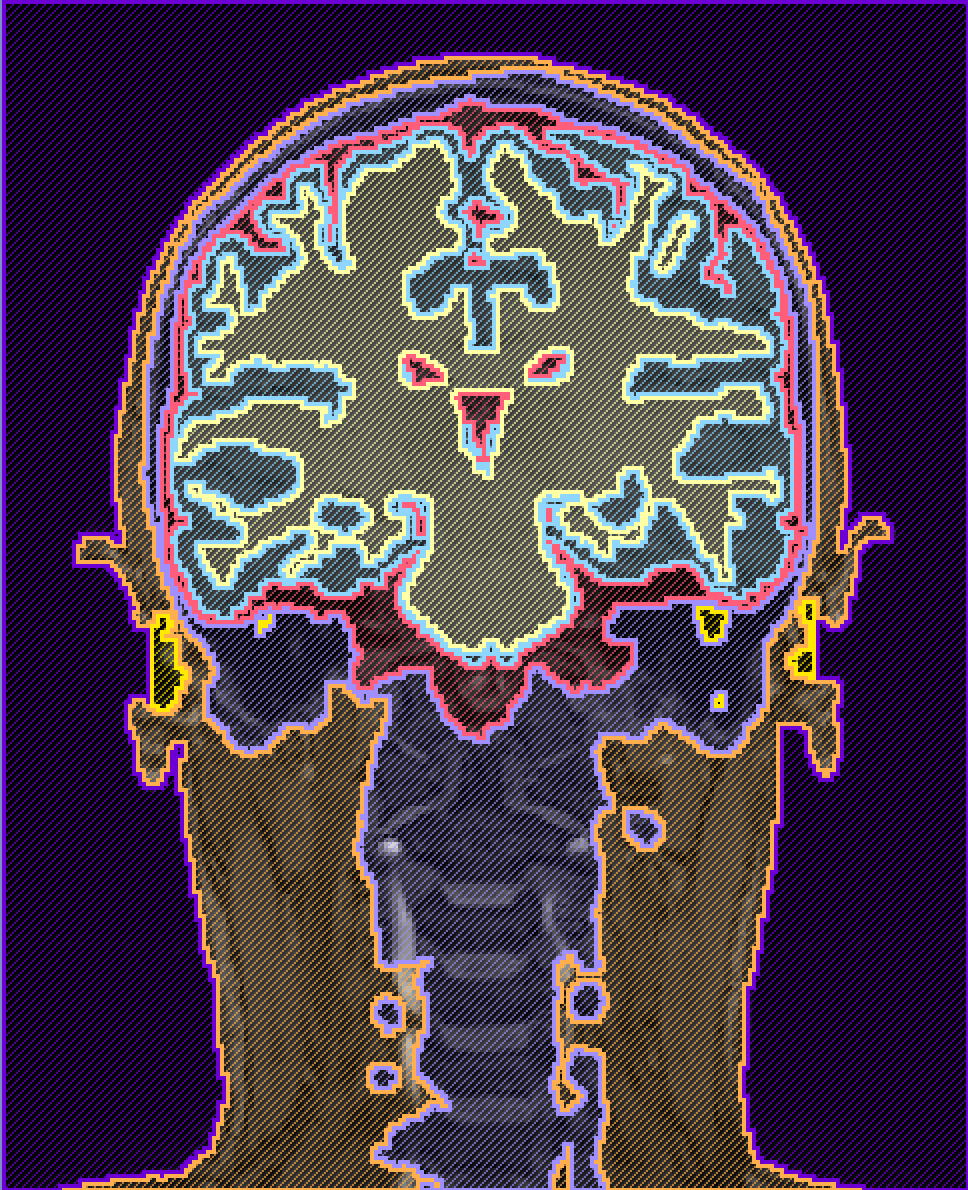
\includegraphics[height=2.35in]{Figures/seg_3}
\caption{A high-resolution, eight-layer, full-head segmentation made with Seg3D.}
\label{fig:fullseg}
\end{center}
\end{figure}

Segmentation of the brain was difficult because of the similar grayscale intensities across different tissues, especially between white and grey matter; thresholding the image produced noisy and incomplete layers (Figure \ref{fig:badseg}). As discussed in Section \ref{sec:Seg}, we used FSL FAST and Seg3D for segmentation. This method, compared with Freesurfer \cite{ref:freesurf}, Statistical Parametric Mapping through Matlab (SPM) \cite{ref:spm}, Atlas Based Classification through 3D Slicer \cite{ref:abc}, and Seg3D methods alone, produced the most qualitatively accurate head and brain segmentation results for this data.

\begin{figure}[H]
\begin{center}
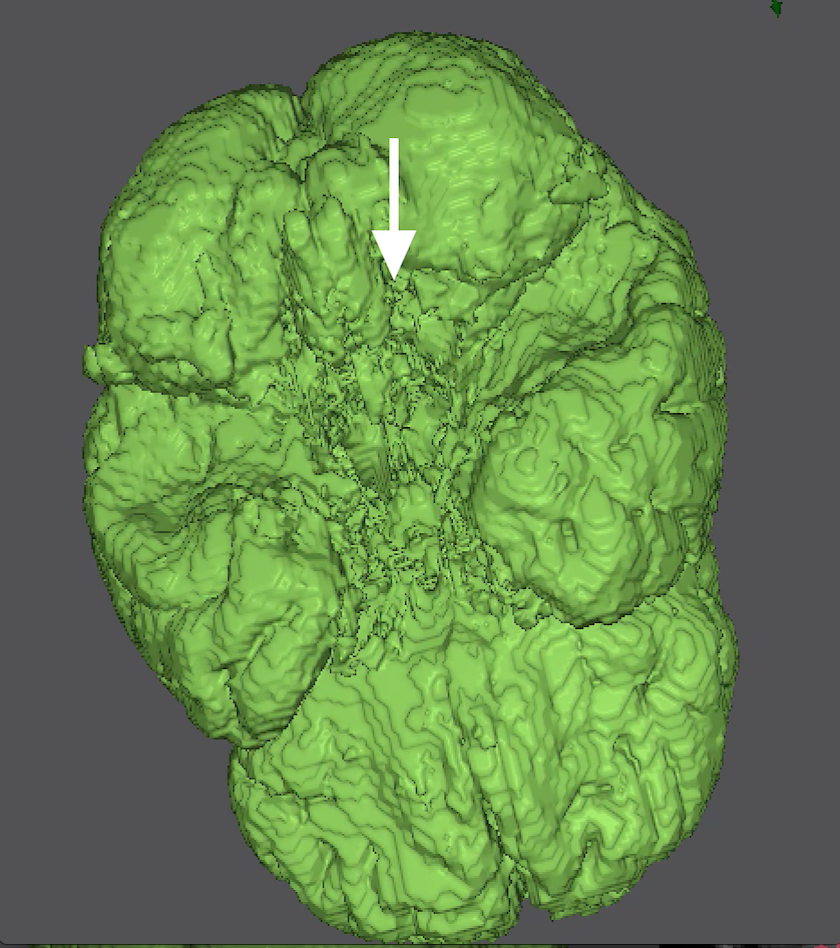
\includegraphics[width=.49\textwidth]{Figures/badseg_1}
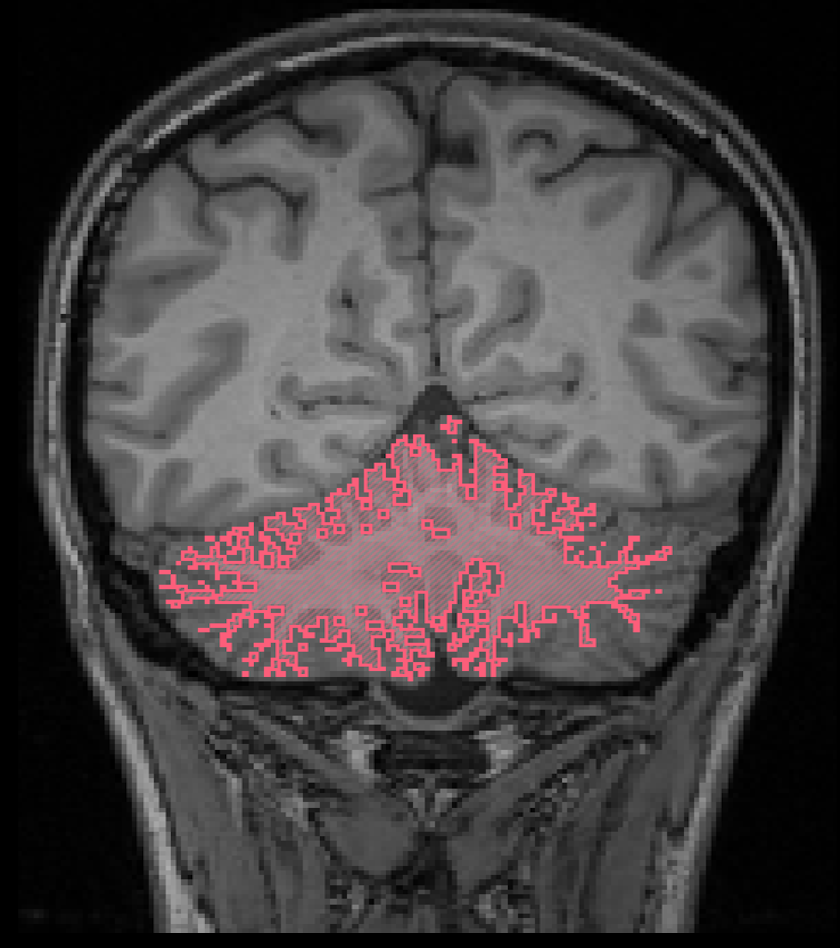
\includegraphics[width=.49\textwidth]{Figures/badseg_2}
\caption{Noisy and incomplete segmentation layers: Isosurface segmentation of gray matter \textit{(left)} and coronal slice of cerebellum segmentation \textit{(right)}. Both segmentations were made using Seg3D.}
\label{fig:badseg}
\end{center}
\end{figure}

The skull and the sinus layers were the most difficult to segment using only an MRI, because they are represented by only black pixels with no clear tissue boundaries, and the subject's data did not include a computed tomography (CT) scan. For our first attempt to create a bone layer, we used FSL's BET2 tool (Figure \ref{fig:bet2}) to extract a skull surface. We then thresholded the $T_1$ MRI to create the remainder of the bones in Seg3D, and connected the bones to the skull made from FSL using a Boolean OR mask filter. Although this approach gave an adequate segmentation for the skull (Figure \ref{fig:skull} - \textit{left}), it did not include important tissues, such as the sinus layer. 

This method compared to the method described in Section \ref{sec:Seg} produced geometries that were similar in some areas, but different in others. The segmentation created using FSL's BET2 and Seg3D was rough and had a clear line of where the two segmentations were connected. It also didn't include a chin or a sinus layer. The segmentation created from the pseudo-CT image was smooth and included a chin (Figure \ref{fig:skull} - \textit{right}) and a sinus layer (Figure \ref{fig:sinus}). However, this segmentation included the inside of the mouth as bone, but as mentioned in Section \ref{sec:Seg} this wasn't concerning for simulations results.

\begin{figure}[H]
\begin{center}
\includegraphics[width=.49\textwidth]{Figures/skull_before}
\includegraphics[width=.49\textwidth]{Figures/skull_after}
\caption{Skull segmentation comparison: Created with BET2 and thresholding \textit{(left)} and with pseudo-CT image \textit{(right)}. Both segmentations were made using Seg3D.}
\label{fig:skull}
\end{center}
\end{figure}

\begin{figure}[H]
\begin{center}
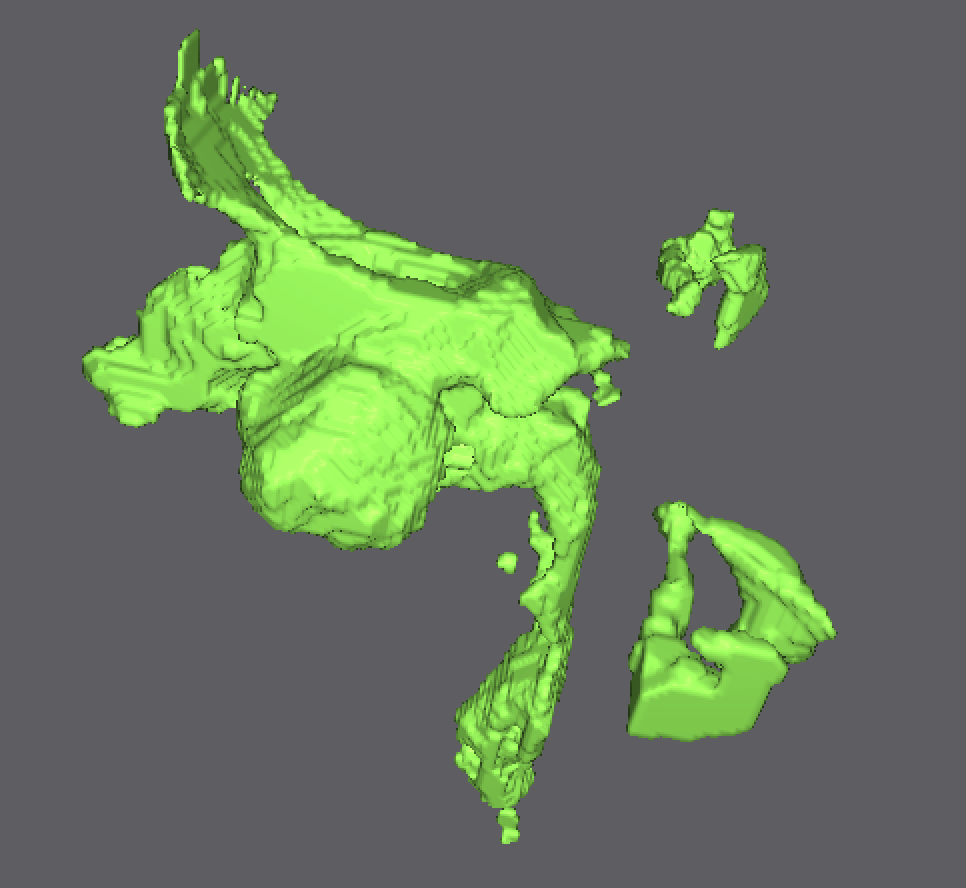
\includegraphics[width=.49\textwidth]{Figures/sinus_iso}
\caption{Sinus segmentation.}
\label{fig:sinus}
\end{center}
\end{figure}

During MRI imaging, the subject was on her back, which caused the brain to shift slightly to the back of the head, causing in thin segmented regions on the back of the head. Other thin segmented regions were on the side of the subject's head, the bridge of the nose, and the bottom of the chin (Figure \ref{fig:thinseg}). We made these sections at least two pixels thick to ensure quality mesh.

\begin{figure}[H]
\begin{center}
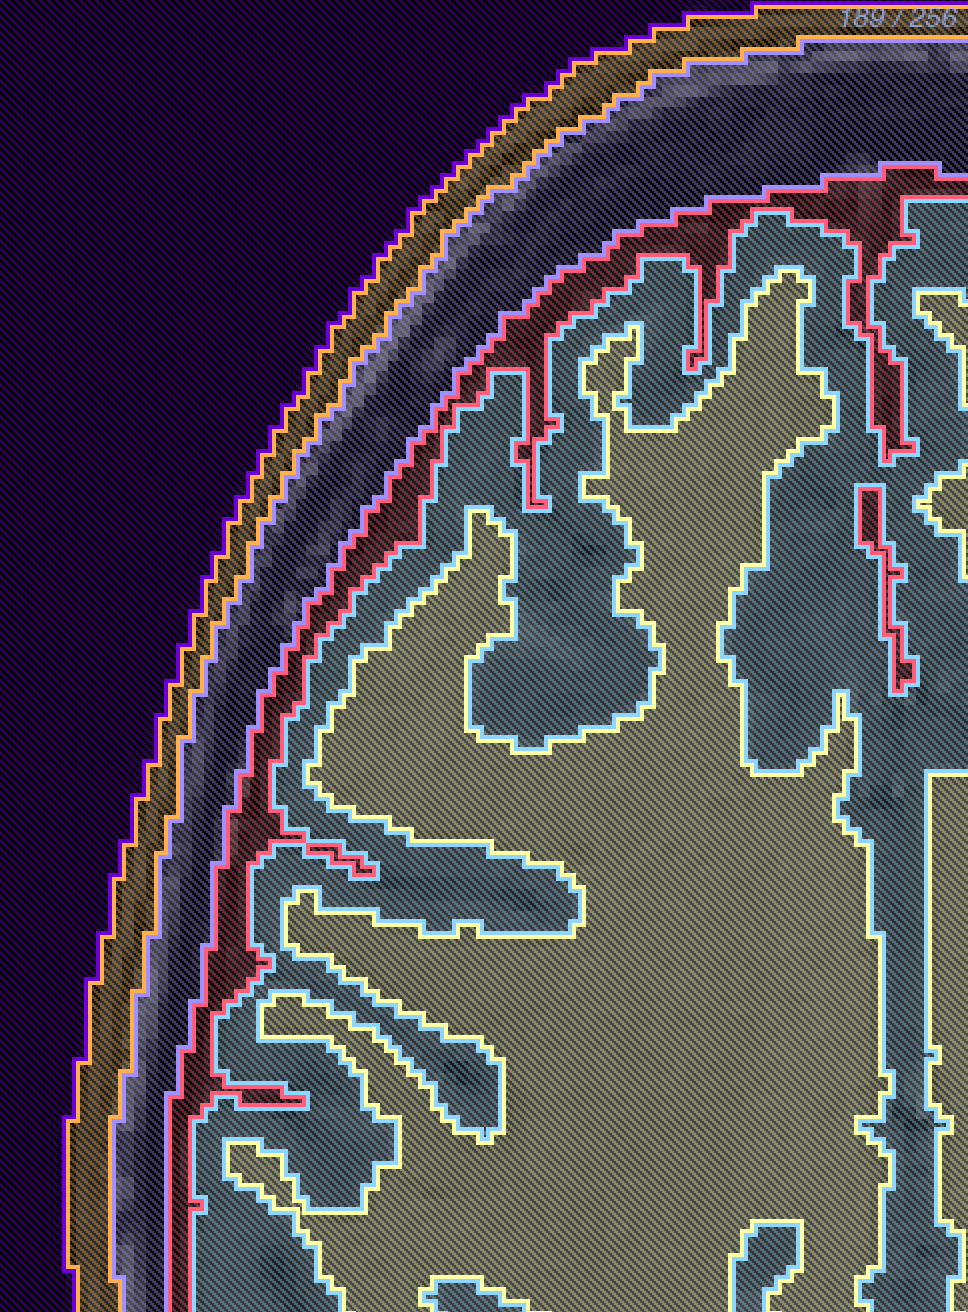
\includegraphics[width=.32\textwidth]{Figures/thin_layer_side}
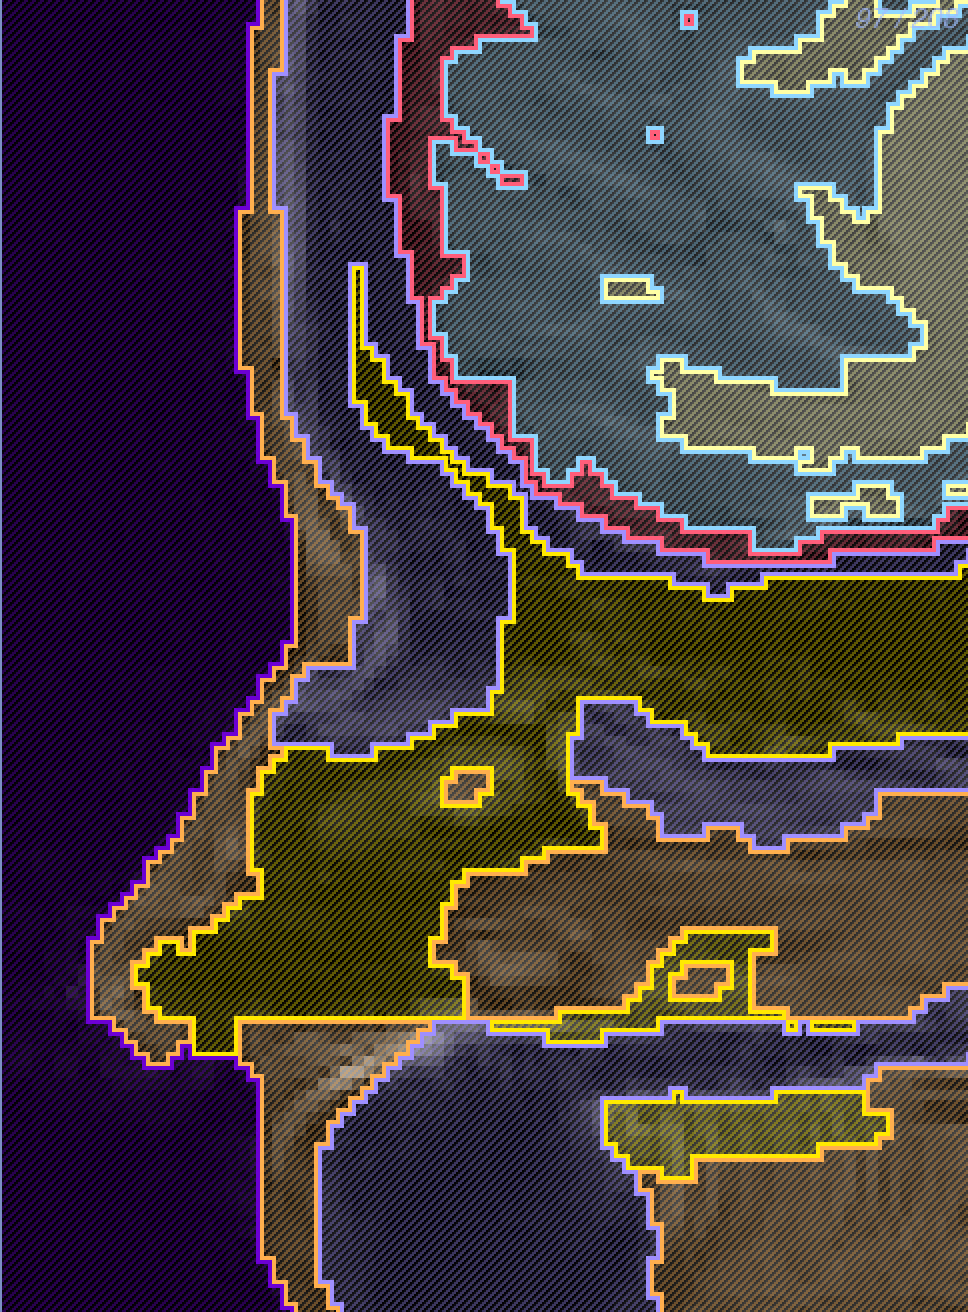
\includegraphics[width=.32\textwidth]{Figures/thin_layer_nose}
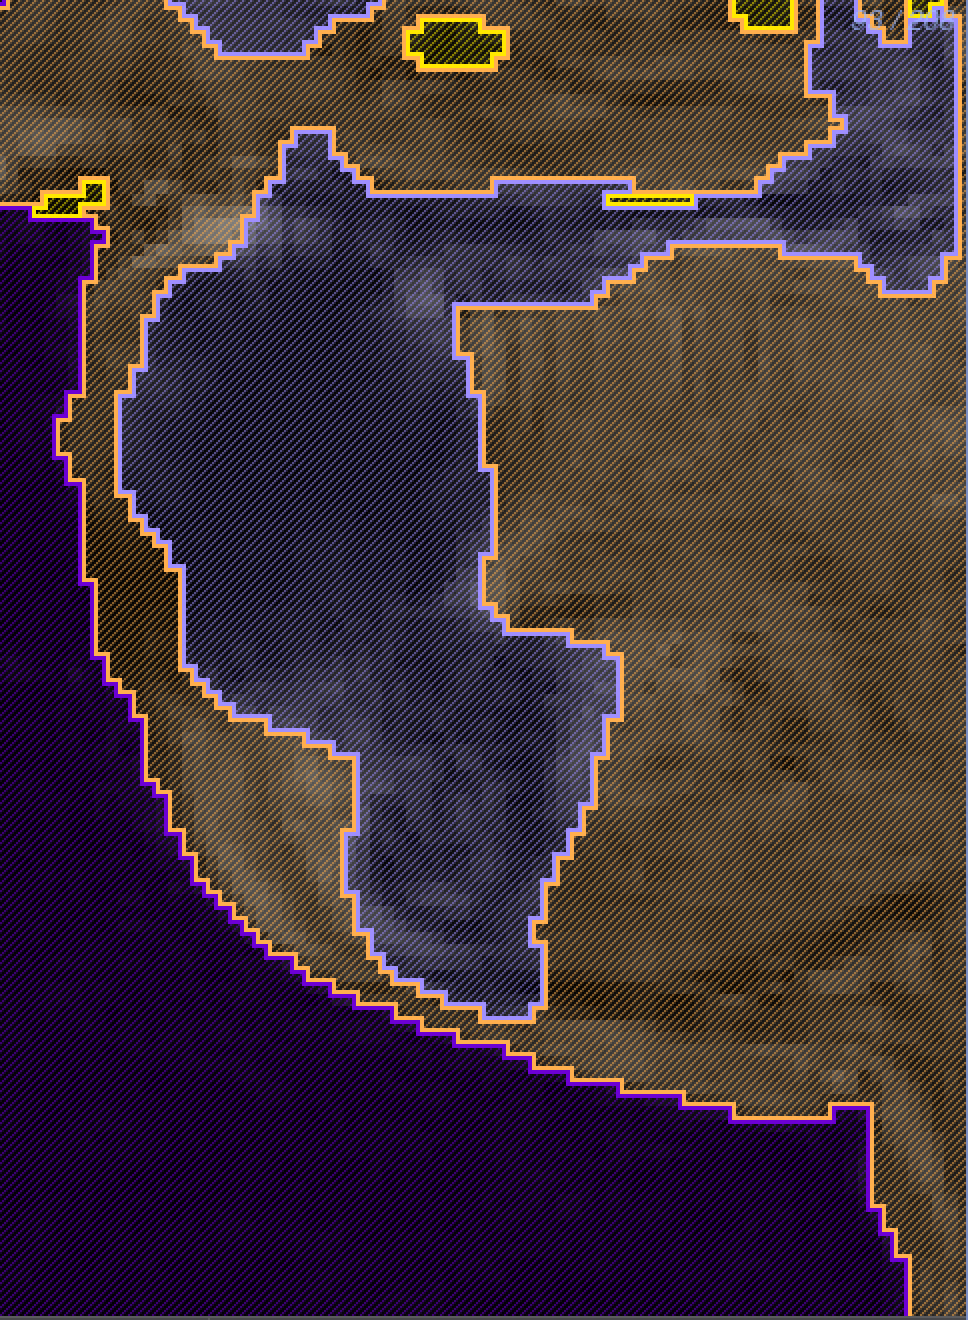
\includegraphics[width=.32\textwidth]{Figures/thin_layer_chin}
\caption{Thin segmentation regions: side of the head \textit{(left)}, bridge of the nose \textit{(middle)}, bottom of the chin \textit{(right)}.}
\label{fig:thinseg}
\end{center}
\end{figure}

\subsection{Finite Element Meshes}

The highest resolution mesh we generated with the settings listed in Section \ref{sec:mesh} contained 60.2 million elements and 10.3 million nodes (Figure \ref{fig:bigmesh}). This mesh was large because of the complexity of the segmentation, including small features, thin sections, and the multi-matieral interface with three or more layers interacting at once. The simulations performed slowly when using this mesh due to its size and required at least 32GB of RAM.

\begin{figure}[H]
\begin{center}
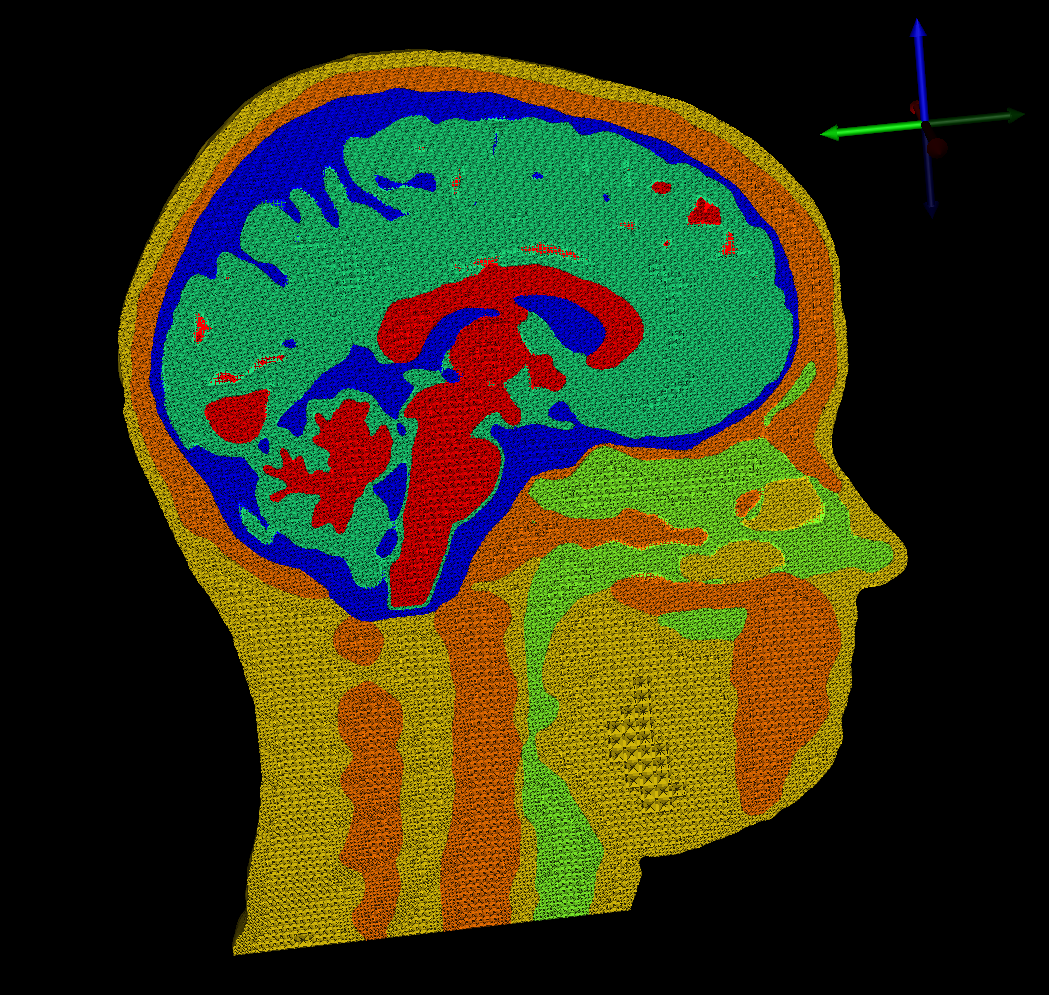
\includegraphics[width=.49\textwidth]{Figures/bigmesh_1}
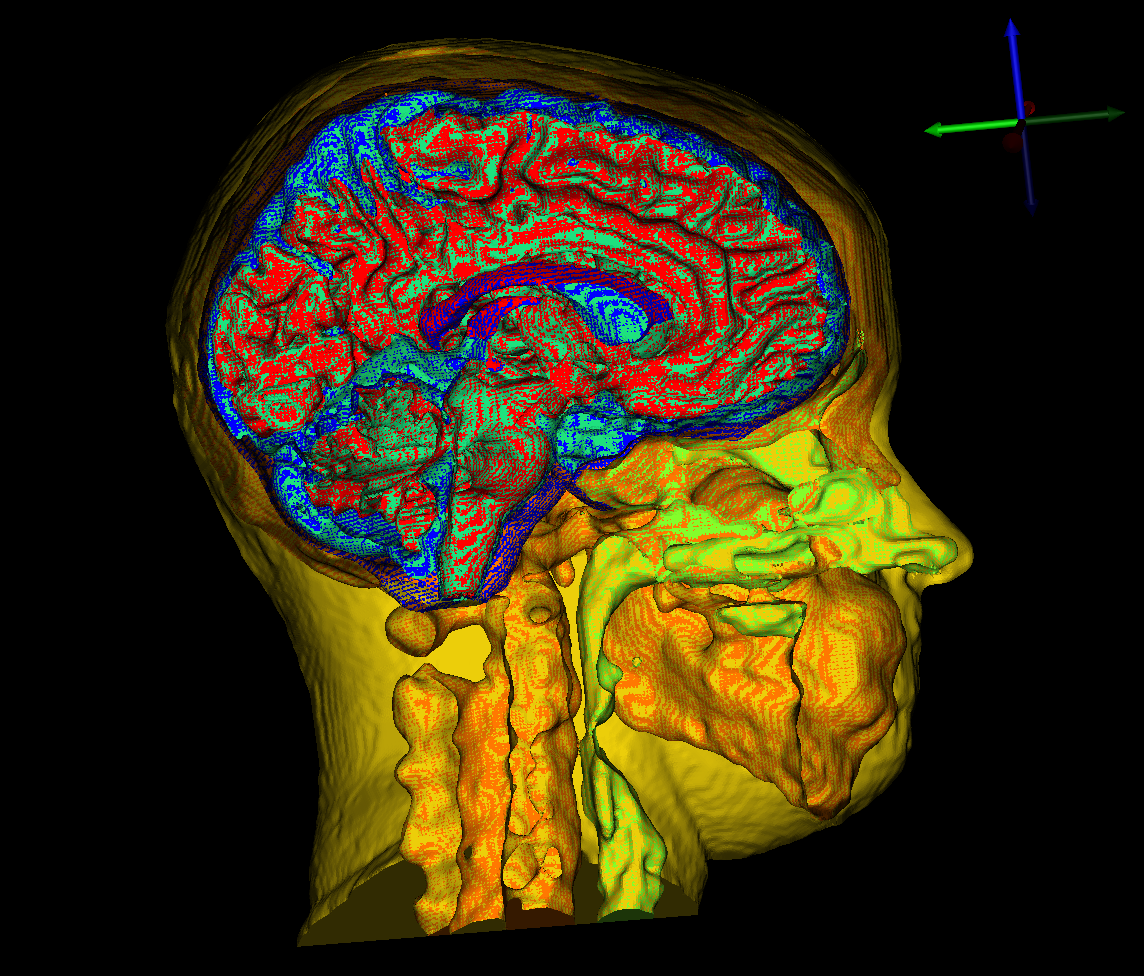
\includegraphics[width=.49\textwidth]{Figures/bigmesh_surface}
\caption{60.2 M element mesh: tetrahedral mesh \textit{(left)}, surface mesh \textit{(right)}.}
\label{fig:bigmesh}
\end{center}
\end{figure}

We attempted to generate smaller meshes to be able to run faster simulations, but many of the meshes contained holes (Figure \ref{fig:meshholes}). After we manually changed the sizing field described in Section \ref{sec:mesh}, we generated a mesh with 15.7 million elements and 2.7 million nodes without holes (Figure \ref{fig:smallmesh}). However, this mesh contained one flat tetrahedra, which we later removed in a SCIRun network (Figure \ref{fig:isofornet} and Figure \ref{fig:anisofornet} ). This issue is currently being investigated by Cleaver software developers.

\begin{figure}[H]
\begin{center}
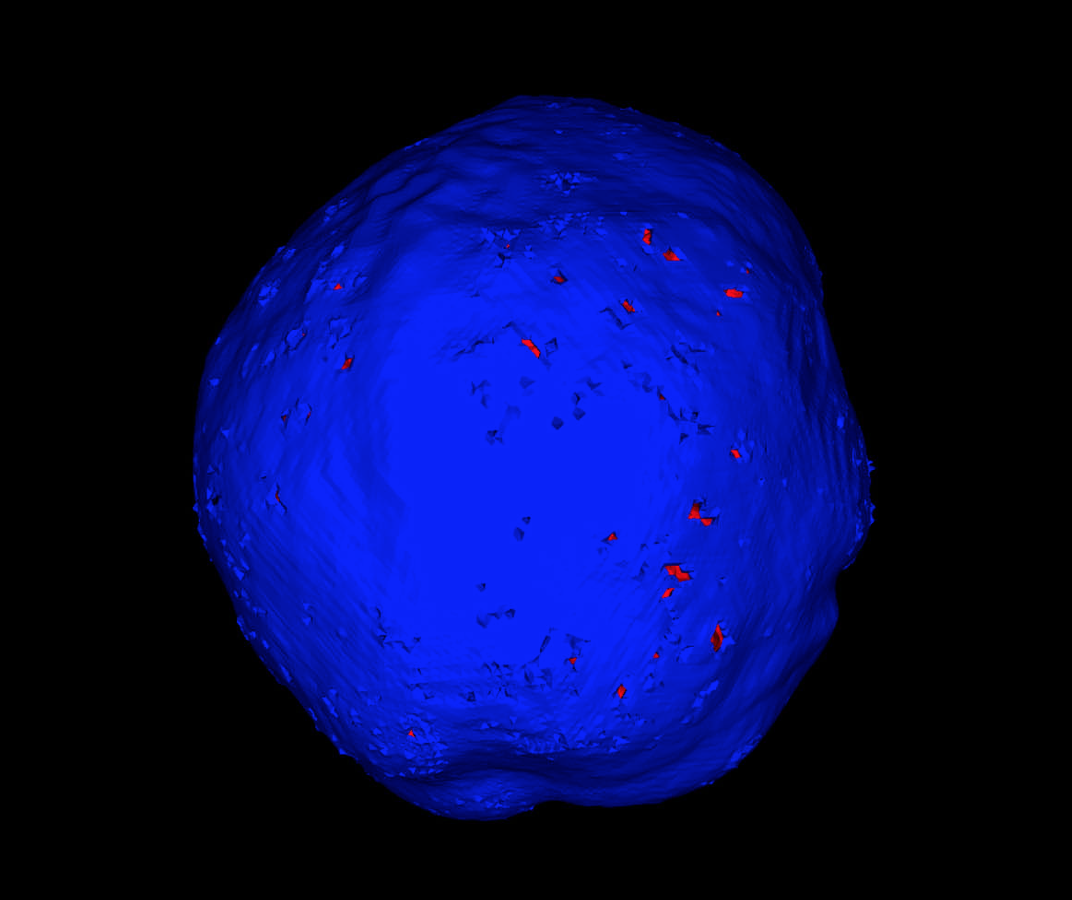
\includegraphics[width=.60\textwidth]{Figures/mesh_with_holes}
\caption{An example of a mesh containing holes.}
\label{fig:meshholes}
\end{center}
\end{figure}

\begin{figure}[H]
\begin{center}
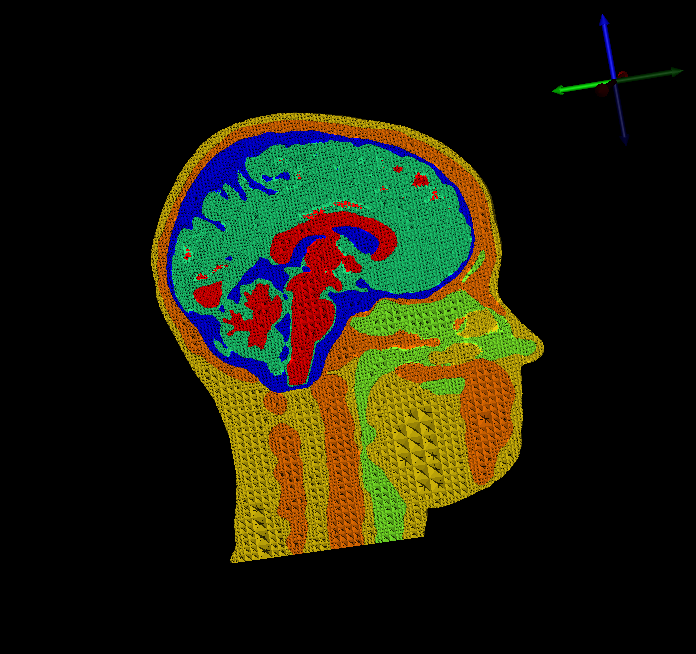
\includegraphics[width=.49\textwidth]{Figures/smallmesh_2}
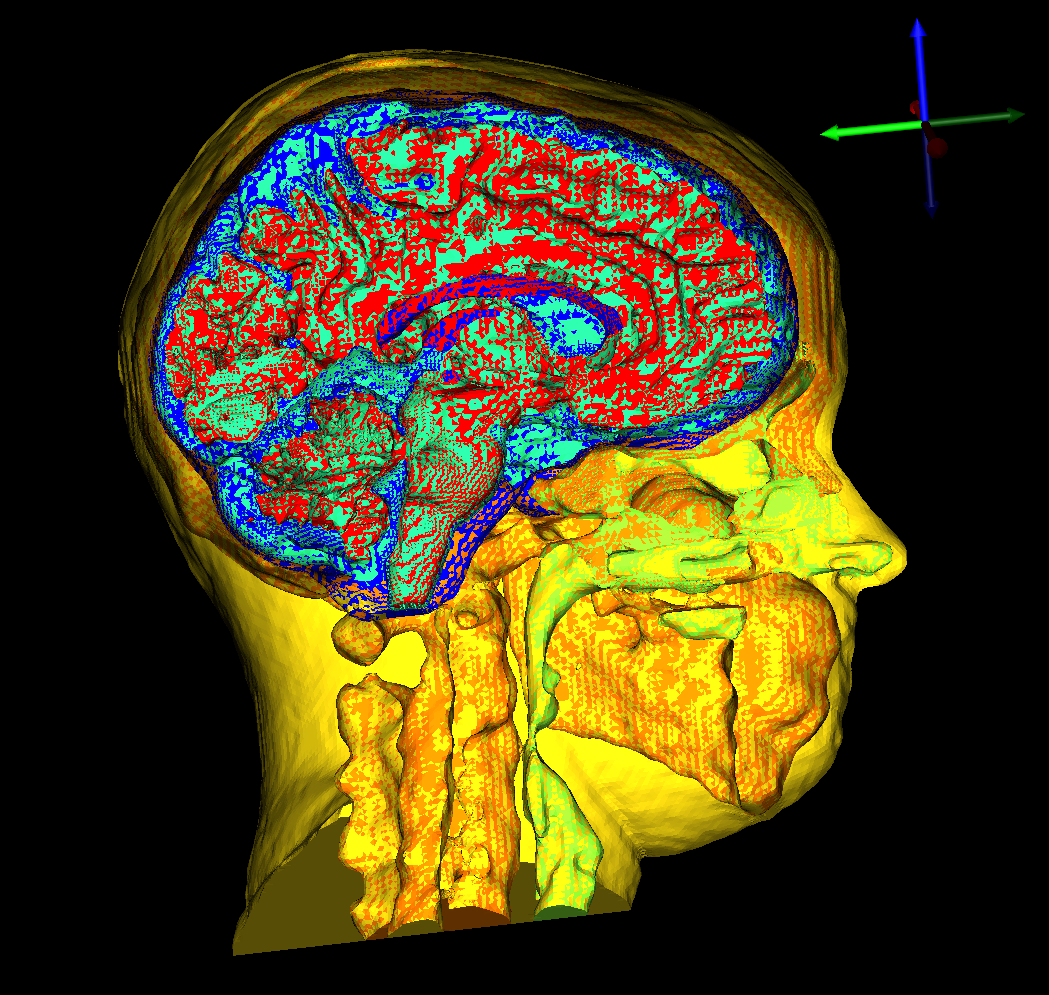
\includegraphics[width=.49\textwidth]{Figures/smallmesh_surface}
\caption{15.7 M element mesh: tetrahedral mesh \textit{(left)}, surface mesh \textit{(right)}.}
\label{fig:smallmesh}
\end{center}
\end{figure}

\subsection{Forward Problem}

\subsubsection{Isotropic}

An isotropic, inhomogeneous head model is expected to have mostly spherical propagation of electrical signals. The simulations showed spherical propagation and acceptable registration of electrodes and dipoles to the mesh space (Figure \ref{fig:isodip}). We generated three-dimensional streamlines (Figure \ref{fig:isostream}) as well as isopotential lines to visualize this propagation and to compare isotropic and anisotropic conductivity (Figure \ref{fig:isolines}). 

\begin{figure}[H]
\begin{center}
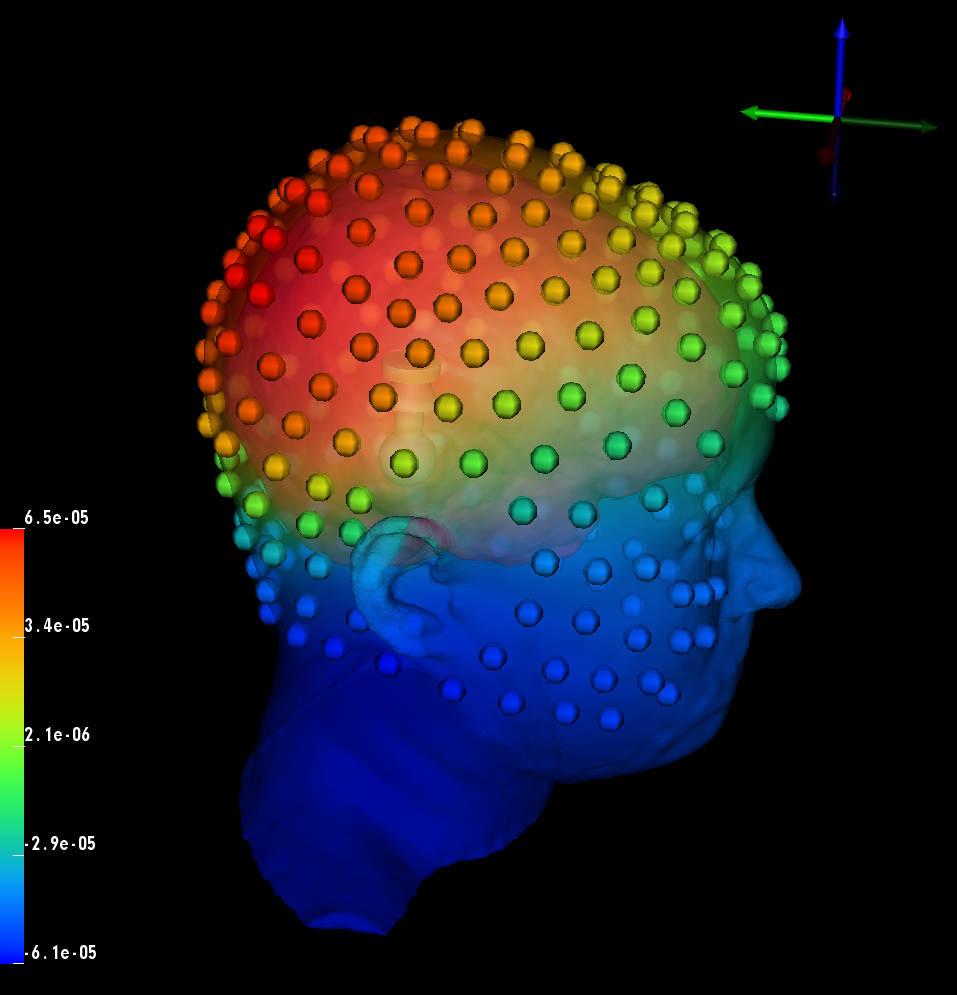
\includegraphics[width=.49\textwidth]{Figures/iso_dipole}
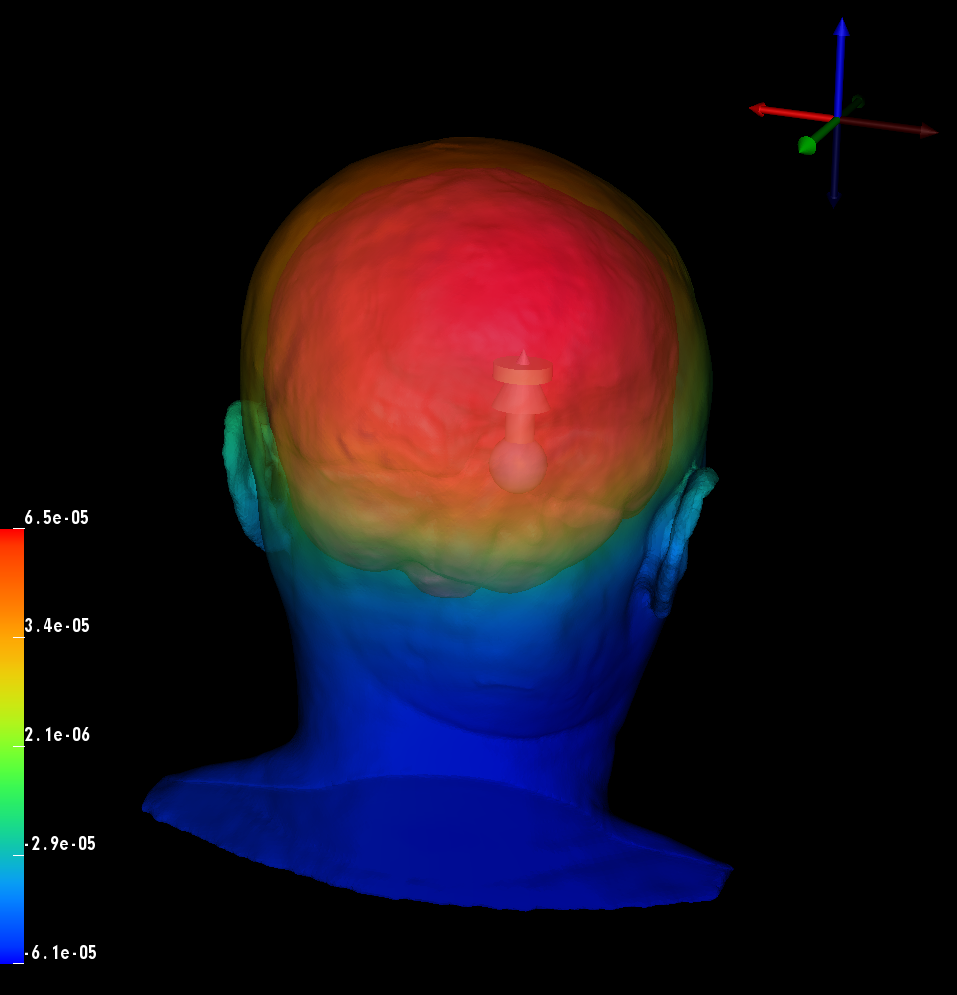
\includegraphics[width=.49\textwidth]{Figures/iso_dipole_2}
\caption{Isotropic forward problem solution with dipole source and data mapped onto the head surface and electrodes.}
\label{fig:isodip}
\end{center}
\end{figure}

\begin{figure}[H]
\begin{center}
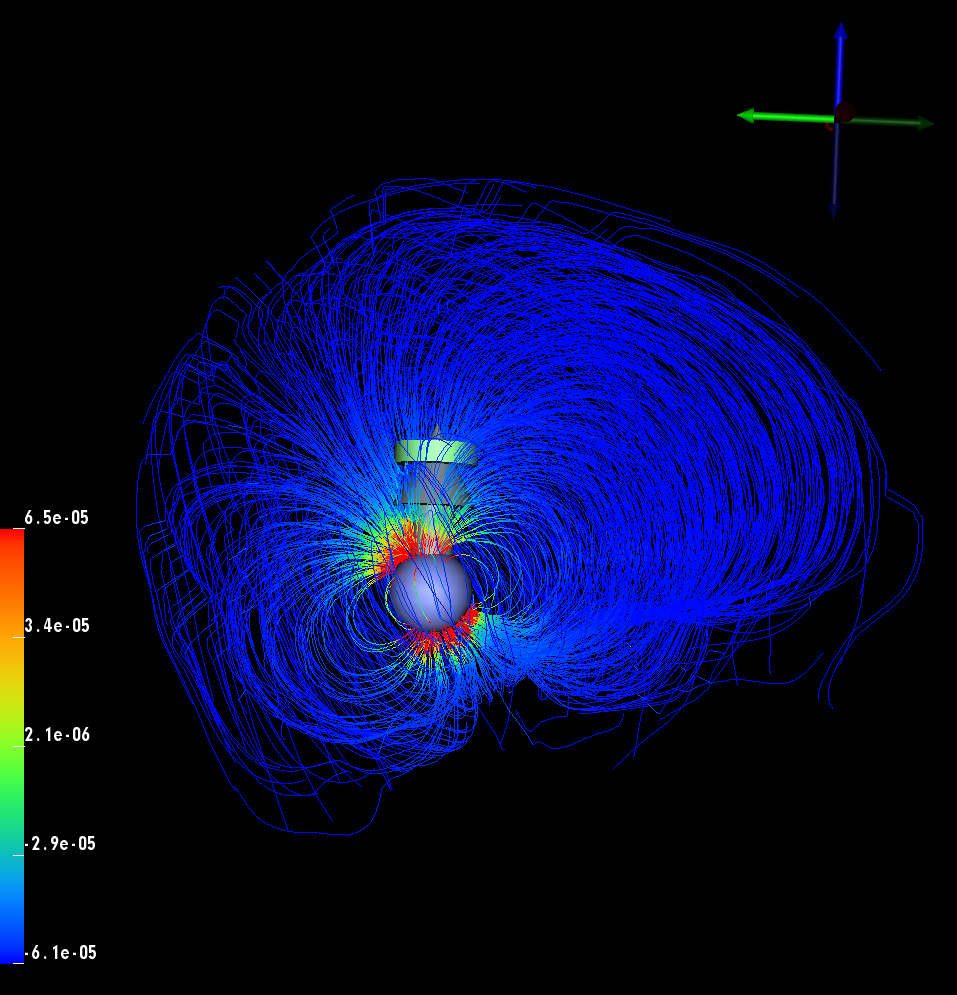
\includegraphics[width=.49\textwidth]{Figures/iso_streamlines}
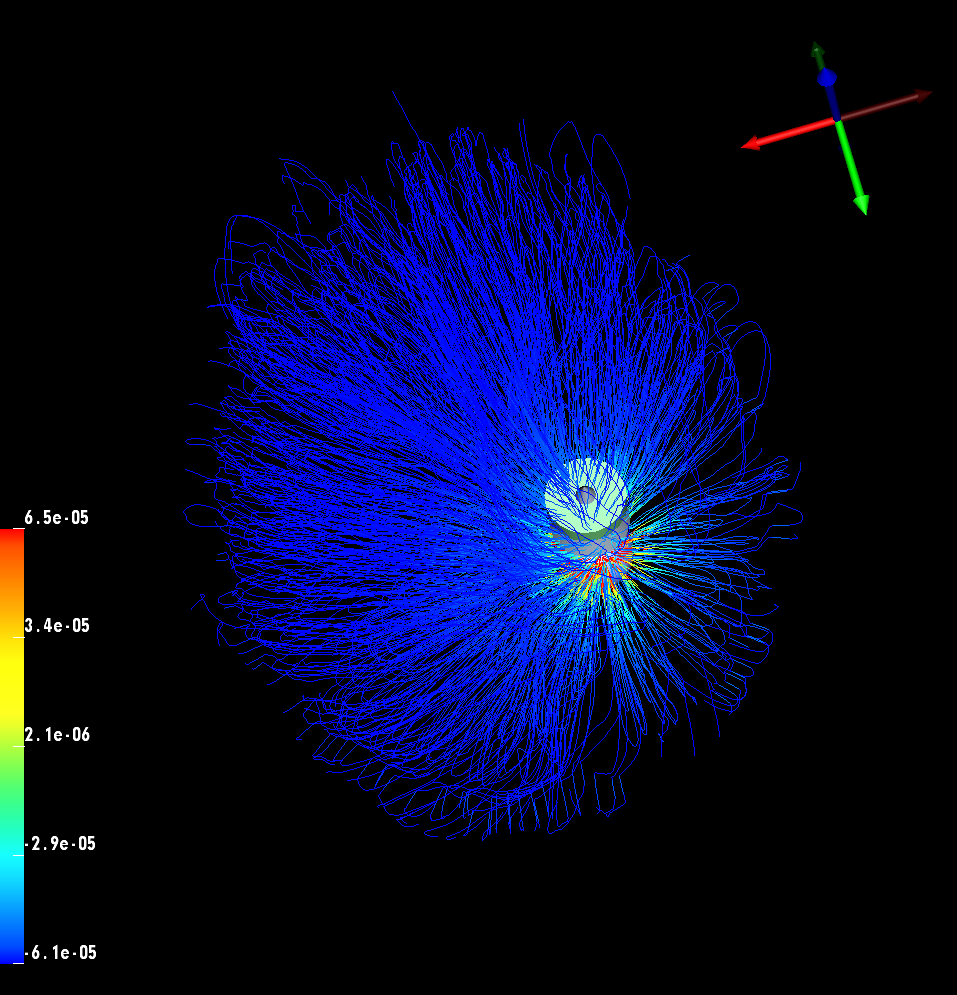
\includegraphics[width=.49\textwidth]{Figures/iso_streamlines_top}
\caption{Isotropic streamlines with dipole source.}
\label{fig:isostream}
\end{center}
\end{figure}

\subsubsection{Anisotropic}

The expectation for an anisotropic, inhomogeneous head model is to have nonspherical propagation, which can be seen with the streamline (Figure \ref{fig:anisostream}) and isopotential line (Figure \ref{fig:isolines}) visualizations. As discussed in Section \ref{sec:cond}, two methods are used for implementing diffusion tensor data, both being available in the SCIRun network shown in Figure \ref{fig:anisofornet}. For Figures \ref{fig:anisodip} - \ref{fig:isolines}, we used the scaling method (equation \ref{eq:scaling}). The simulations showed nonspherical propagation and acceptable registration of the electrodes, dipoles, and mesh into the diffusion tensor space (Figure \ref{fig:anisodip}).

\begin{figure}[H]
\begin{center}
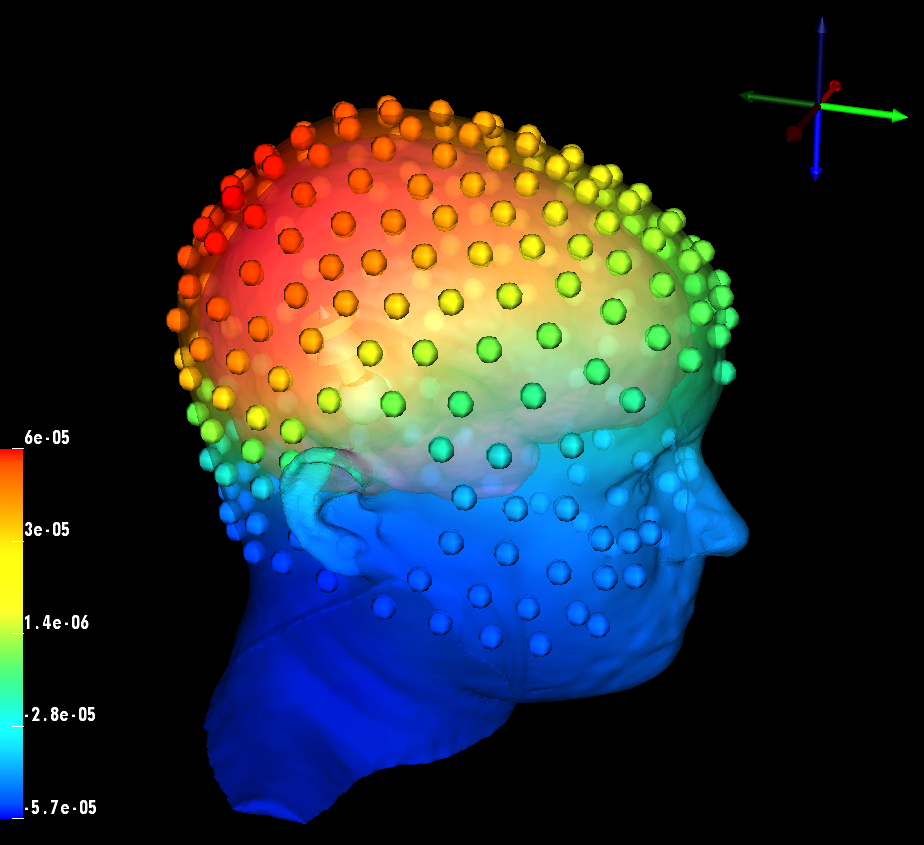
\includegraphics[width=.49\textwidth]{Figures/aniso_dipole}
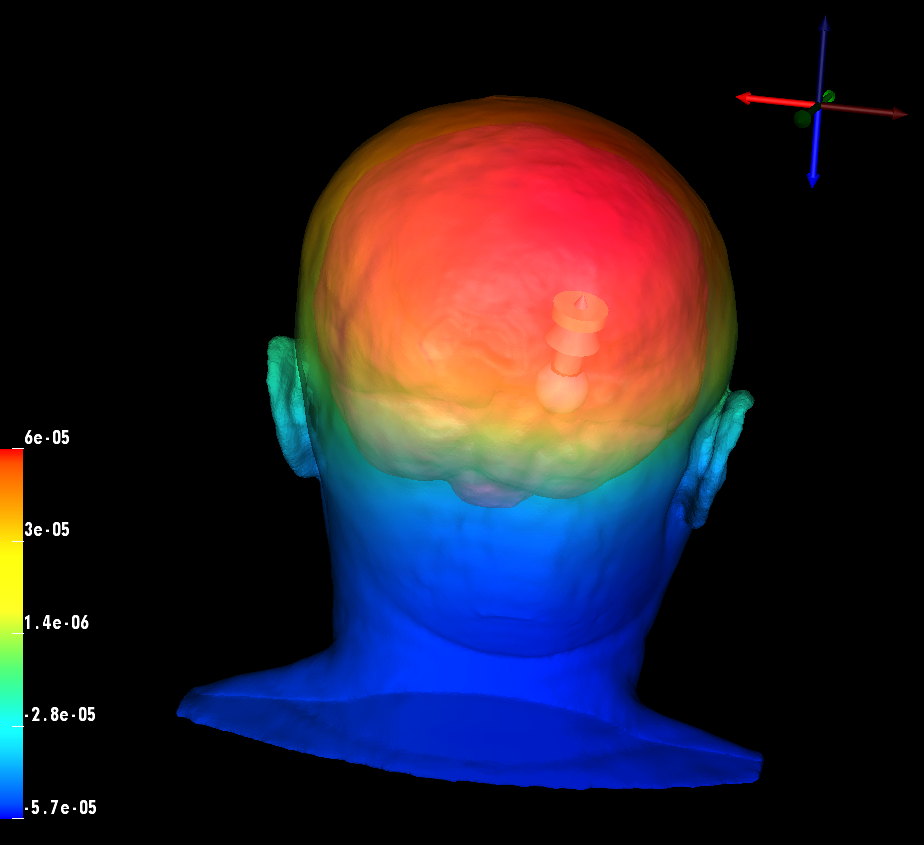
\includegraphics[width=.49\textwidth]{Figures/aniso_dipole_2}
\caption{Anisotropic forward problem solution with dipole source and data mapped onto the head surface and electrodes.}
\label{fig:anisodip}
\end{center}
\end{figure}

\begin{figure}[H]
\begin{center}
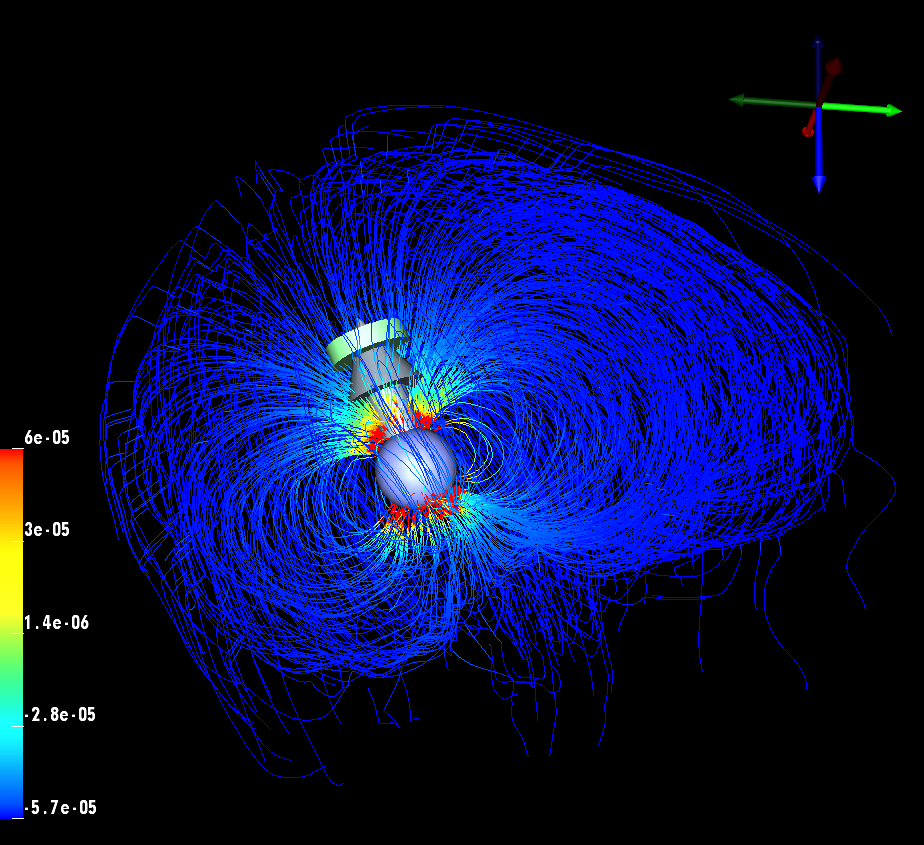
\includegraphics[width=.49\textwidth]{Figures/aniso_streamlines}
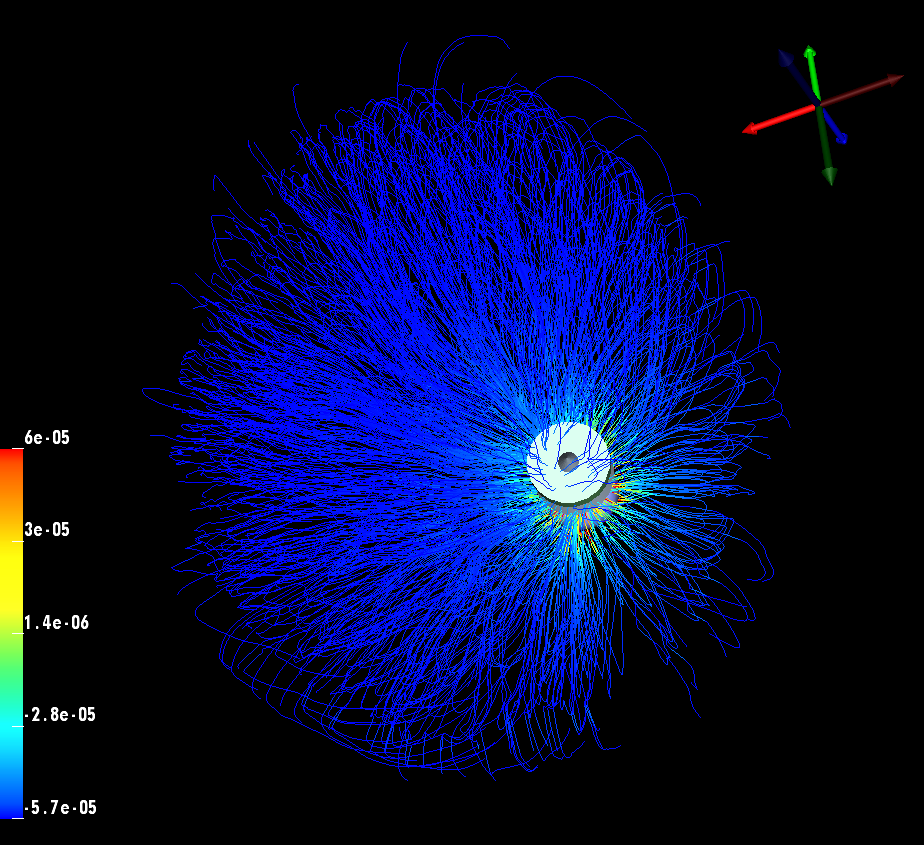
\includegraphics[width=.49\textwidth]{Figures/aniso_streamlines_top}
\caption{Anisotropic streamlines visualization with dipole source.}
\label{fig:anisostream}
\end{center}
\end{figure}

\begin{figure}[H]
\begin{center}
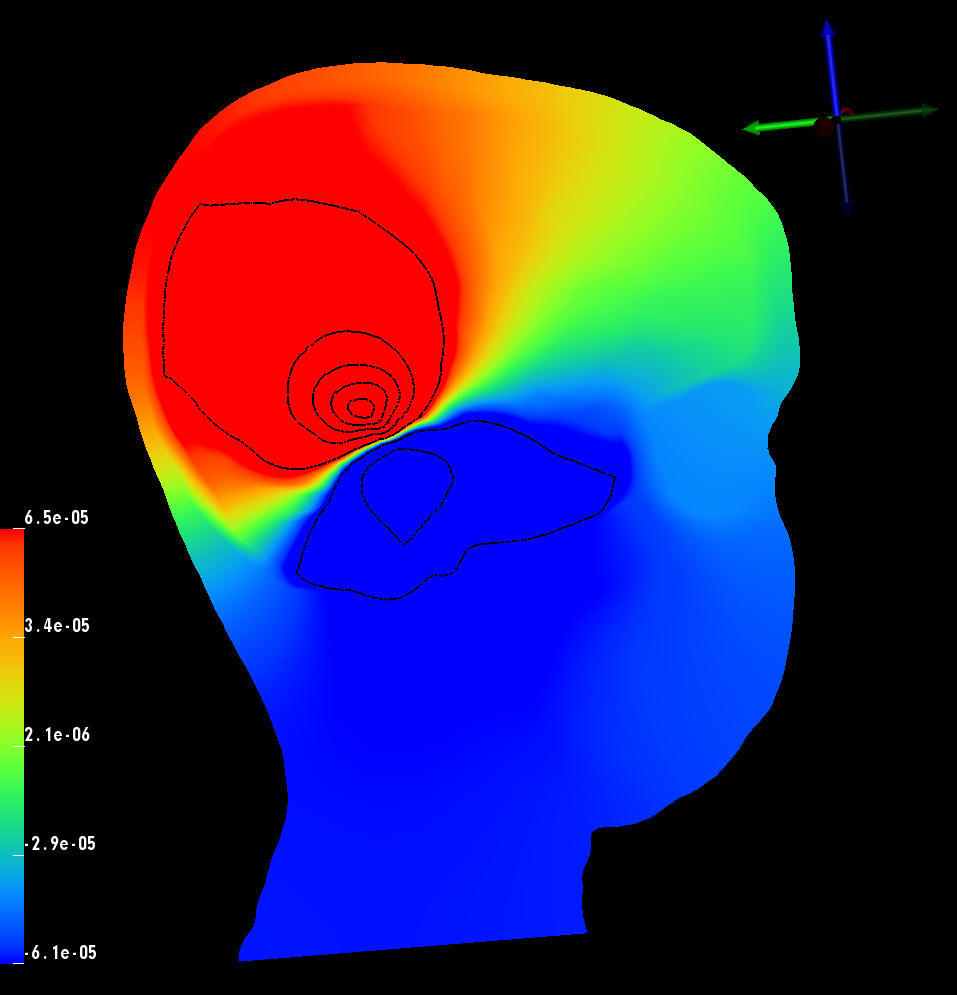
\includegraphics[width=.49\textwidth]{Figures/iso_isolines}
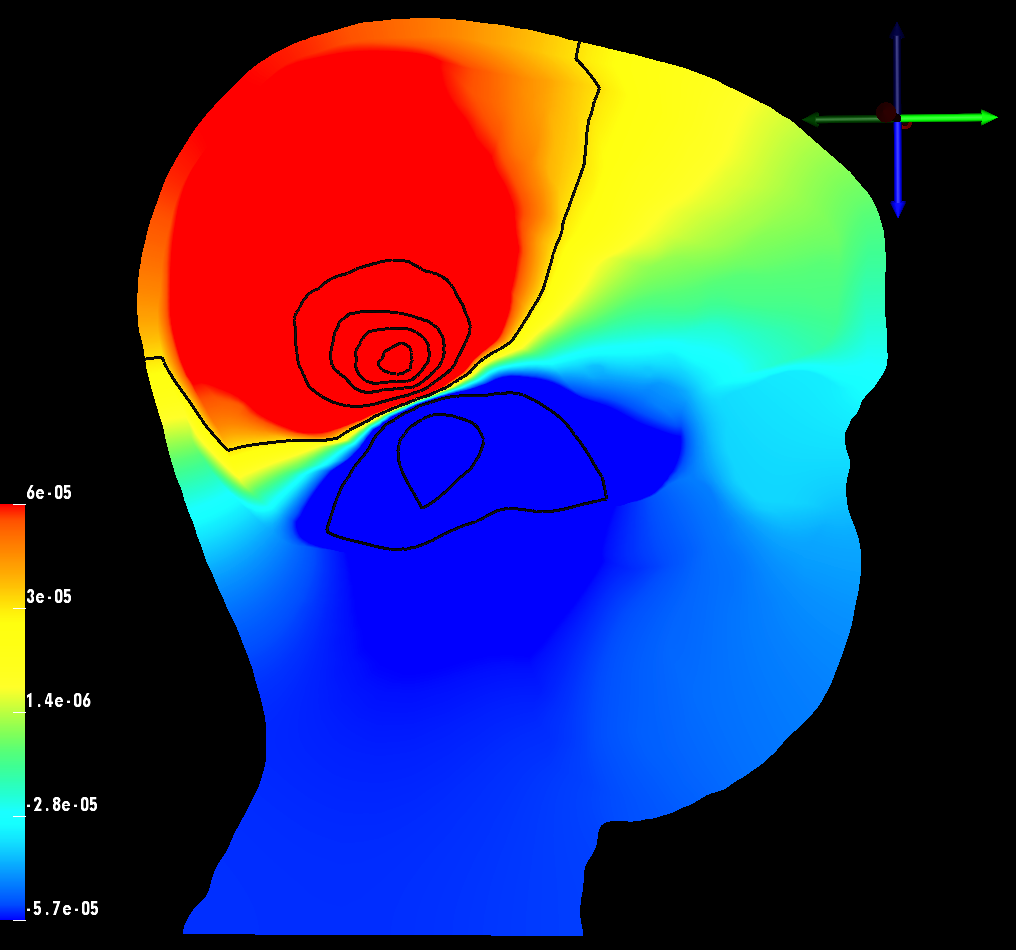
\includegraphics[width = .49\textwidth]{Figures/aniso_isolines}
\caption{Isopotential lines comparison: isotropic white matter conductivity \textit{(left)}, anisotropic white matter conductivity \textit{(right)}.}
\label{fig:isolines}
\end{center}
\end{figure}

\subsection{fMRI Visualization}

fMRI data was a novel imaging datatype for SCIRun. We successfully mapped and visualized the fMRI data onto the cortical surface with a rigid and manual registration, as discussed in Section \ref{sec:reg}, to the mesh coordinate space (Figure \ref{fig:fmrivis}). This mapping network allows for future use of fMRI data in simulations using SCIRun (Figure \ref{fig:fmrivisnet}). The manual registration we applied is fairly accurate since we didn't see any large patches of zero signal, which would appear in blue. We also saw the higher signals on the brain stem, which has the most blood flow.

\begin{figure}[H]
\begin{center}
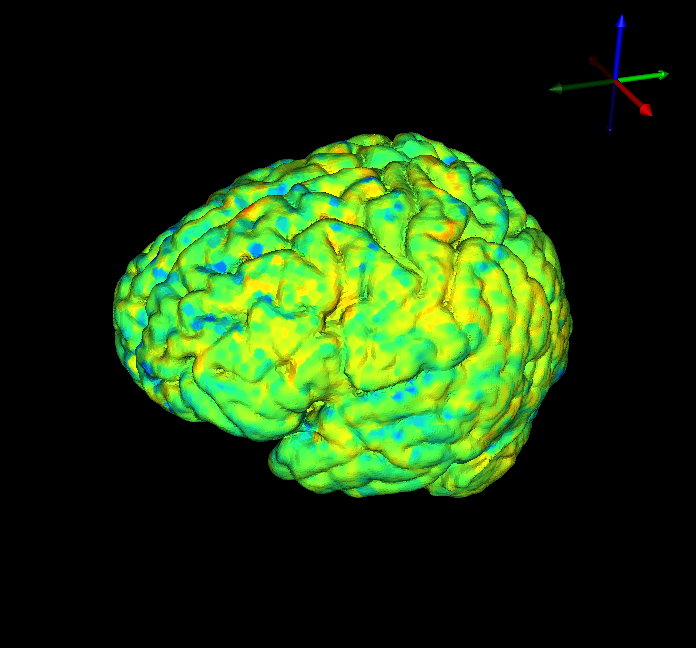
\includegraphics[width=.75\textwidth]{Figures/fmri_1}
\caption{fMRI data mapped onto cortical surface mesh.}
\label{fig:fmrivis}
\end{center}
\end{figure}

\subsection{EEG Visualization}

When using EEG data, the particular application dictates if further processing, filtering, or cutting of the data is necessary. This EEG dataset, taken with 256 electrodes, contained electrodes that require further processing, specifically around the eyes, which was possibly due to the blinking or rolling of the subject's eyes. These electrodes can be corrected or removed with further specific processing such as trilinear interpolation.

\begin{figure}[H]
\begin{center}
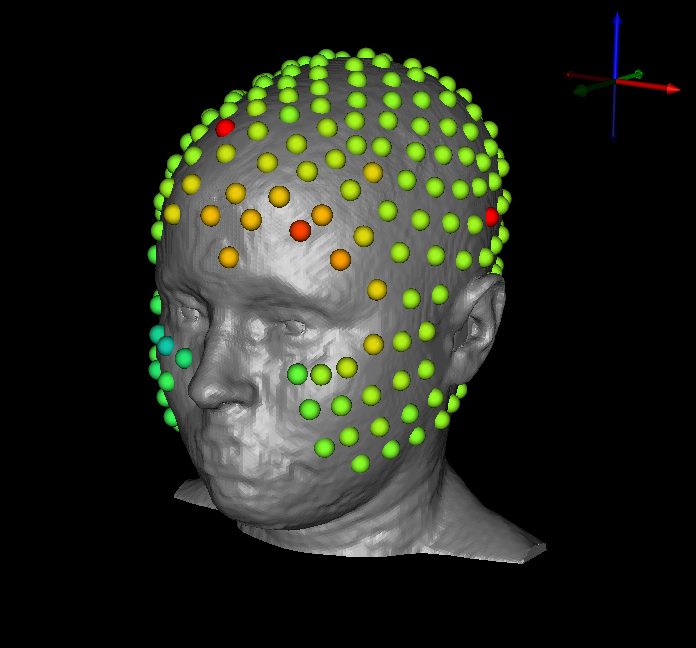
\includegraphics[width=.49\textwidth]{Figures/eeg_1}
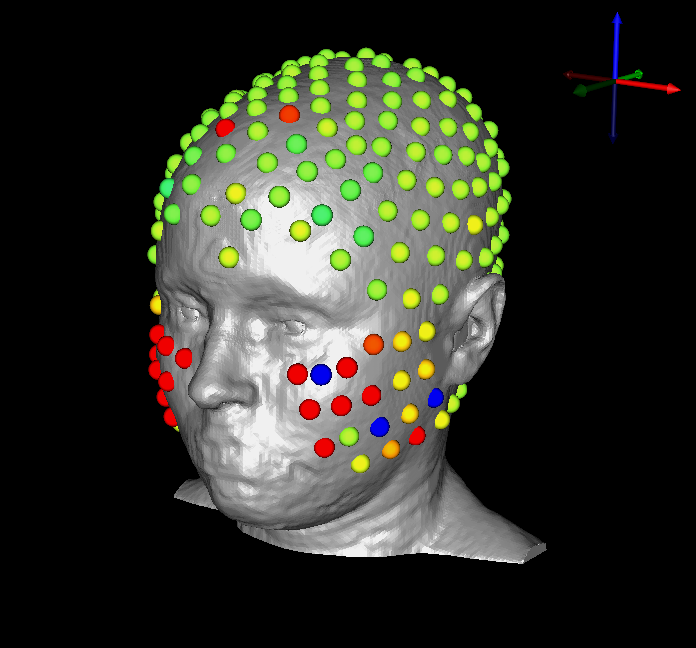
\includegraphics[width=.49\textwidth]{Figures/eeg_2}
\caption{EEG signal visualization with 256 electrodes. Examples of electrodes that require further processing for specific applications - shown in red.}
\label{fig:eegvis}
\end{center}
\end{figure}

The second EEG dataset, taken with 128 electrodes, also contains electrodes that require further processing around the eyes (Figure \ref{fig:eegvis}). Since the electrodes don't go as far down the cheeks as the other dataset, we do not see as many of these electrodes. However, the quality of some time steps were too poor for practical use and can be removed.

\begin{figure}[H]
\begin{center}
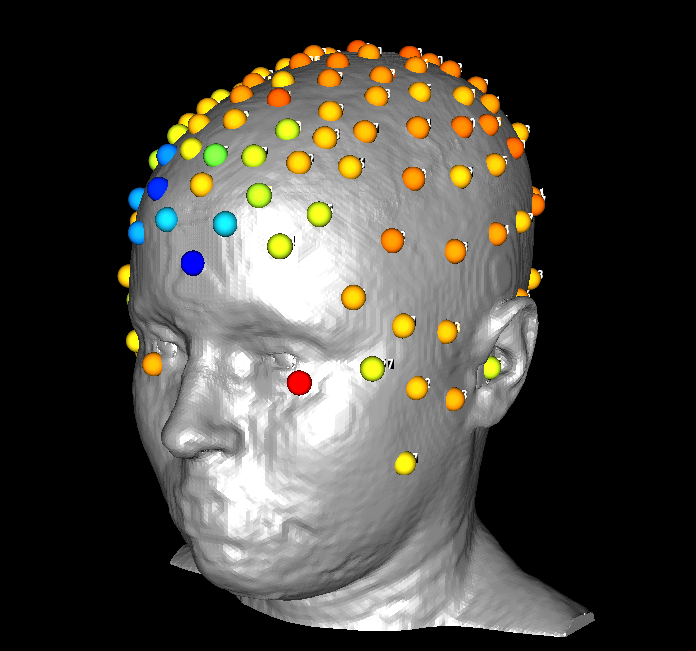
\includegraphics[width=.49\textwidth]{Figures/128_eeg_1}
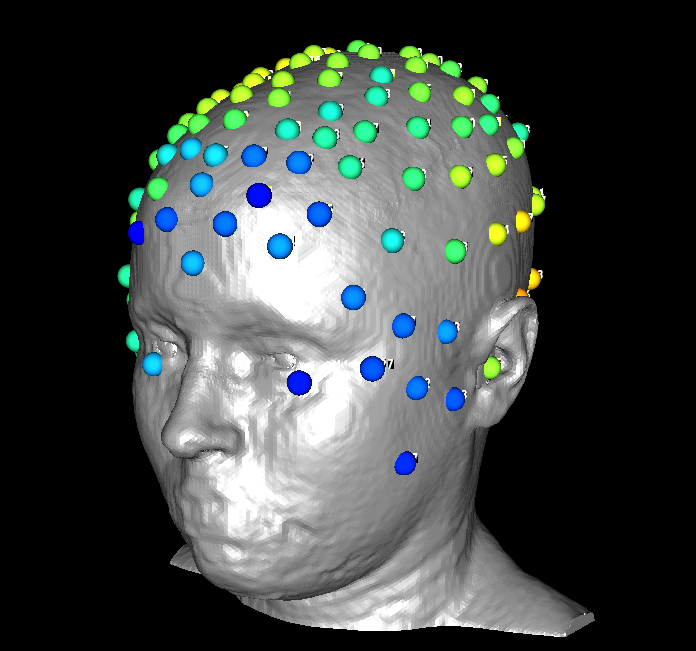
\includegraphics[width=.49\textwidth]{Figures/128_eeg_2}
\caption{EEG signal visualization with 128 electrodes. Examples of electrodes that require further processing for specific applications - shown in red.}
\label{fig:eegvis}
\end{center}
\end{figure}

The manual registration we applied to the electrodes is fairly accurate, as well. The spaces for the ears and eyes are where we expected them, and fit to the surface of the head mesh without any gapping or shifting. 

\subsection{Future Investigations Discussion}

Future investigations based on this pipeline include finding more appropriate decimation algorithms for three-dimensional tetrahedral finite element meshes to further reduce the mesh size; more exact sinus and skull segmentation methods to improve the appearance and accuracy of these layers; and more robust registration techniques, which will provide a better transformation matrix for moving images to DTI coordinate space, especially for fMRI data. Additions to this dataset could include more methods to incorporate fMRI data into source localization forward and inverse simulations and more specific processing of EEG data for different applications, resulting in more accurate and realistic visualizations. 


